\documentclass[12pt,a4paper]{report}
\usepackage[utf8]{inputenc}
\usepackage{amsmath}
\usepackage{amsfonts}
\usepackage{amssymb}
\usepackage{graphicx}
\usepackage[framemethod=TikZ]{mdframed}
\usepackage{mathtools,tikz-cd}
\usepackage{epstopdf}
\usepackage{xcolor}
\usepackage{mdframed}
\usepackage[english]{babel}
\usepackage[left=3.50cm, right=2.00cm, top=3.00cm, bottom=3.50cm]{geometry}
\renewcommand{\baselinestretch}{1.5}
\renewcommand{\footnotesize}{\fontsize{13pt}{1}\selectfont}
%\usepackage[margin=1in]{geometry}  % set the margins to 1in on all sides
\usepackage{graphicx}              % to include figures
\usepackage{amsmath}               % great math stuff
\usepackage{amsfonts}              % for blackboard bold, etc
\usepackage{amsthm}                % better theorem environments
\usepackage{fancyhdr}
\usepackage{enumitem}
\usepackage{mathtools,etoolbox}
\usepackage{mathrsfs}
\usepackage{relsize}%
\usepackage{makecell}
\usepackage{tabularx,colortbl}
\usepackage{pgfplots}
\usepackage{wrapfig}
\usepackage{braket}
\usepackage{float}
\usepackage{cases}
\usepackage{tabto}
\usepackage{longtable}
\usepackage[english]{babel}
\usepackage{mdframed}
\usepackage{lipsum}
\usepackage[none]{hyphenat}
\usepackage{fancyhdr}
\usepackage{listings}
\usepackage[caption = false]{subfig}
\usepackage[driverfallback=hypertex]{hyperref}
\usepackage[nottoc]{tocbibind}
\usepackage{pbox}
\usepackage{makecell}
\usepackage{tcolorbox}
\usepackage{url}
\usepackage{tikz}
\tikzset{point/.style={circle,draw=black,inner sep=0pt,minimum size=3pt}}
\usetikzlibrary{calc}
\usetikzlibrary{positioning}
\usetikzlibrary{quotes,arrows.meta}
\usetikzlibrary{shapes,arrows,arrows,positioning,fit}
\usetikzlibrary{arrows,shapes,positioning,shadows,trees}
\floatstyle{ruled} 
\newfloat{Algorithm}{htbp}{loa} 
\floatname{Algorithm}{Algorithm}
\urlstyle{same}
\allowdisplaybreaks
\usepackage{multirow}
\usepackage[titletoc]{appendix}
\usepackage{relsize}
\usepackage{array}
\newcolumntype{P}[1]{>{\hspace{0pt}}p{#1}}
%-----------------------EQUATION------------------------------------------------%
\usepackage{chngcntr}
\counterwithout{equation}{chapter} % cho công thức toán học

%-----------------------EXAMPLE------------------------------------------------%

\usepackage{lmodern}
\usepackage{amssymb,amsthm}
\newcounter{example}
\newenvironment{example}[1][]{\refstepcounter{example}\par\medskip
	\noindent \textbf{Example~\theexample #1} \rmfamily}{\medskip}

%------------------------SOLUTION---------------------------------------------------------%

\newenvironment{solution}
{\let\oldqedsymbol=\qedsymbol
	\renewcommand{\qedsymbol}{$\blacksquare$}
	\begin{proof}[\bfseries\upshape Solution]}
	{\end{proof}
	\renewcommand{\qedsymbol}{\oldqedsymbol}}


%---------------------------------------------------------------------------------%%
\hypersetup{
	colorlinks=true,
	linkcolor=black,
	citecolor=black,
	filecolor=black,
	urlcolor=black,
}

%-------------------------- CODE MATLAB ------------------------------------------------------%
\usepackage{listings}
\usepackage{color} % tô màu cho code	
\definecolor{dkgreen}{rgb}{0,0.6,0}
\definecolor{gray}{rgb}{0.5,0.5,0.5}
\definecolor{mauve}{rgb}{0.58,0,0.82}
\lstset{frame=tb,
	language=Matlab,
	aboveskip=3mm,
	belowskip=3mm,
	showstringspaces=false,
	columns=flexible,
	basicstyle={\small\ttfamily},
	numbers=none,
	numberstyle=\tiny\color{gray},
	keywordstyle=\color{blue},
	commentstyle=\color{dkgreen},
	stringstyle=\color{mauve},
	breaklines=true,
	breakatwhitespace=true,
	tabsize=3
	}
%---------------------------REFERENCES-----------------------------------------------------%	
\usepackage[backend = bibtex, sorting = nty , style = ieee]{biblatex}
\addbibresource{mybibtex.bib}

%---------------------------NUMBER PAGES-----------------------------------------------------%
%\usepackage{fancyhdr}
%\pagestyle{fancy}
%\fancyhf{}
%\chead{\thepage}
%\pagestyle{fancy}
%\fancyhf{}
%\fancyhead[C]{\thepage}
%\fancypagestyle{plain}{%
%	\renewcommand{\headrulewidth}{0pt}%
%	\fancyhf{}%
%	\fancyhead[C]{\thepage}%
%}
%\renewcommand{\headrulewidth}{0pt}%

%------------------------ALGORITHM----------------------------------------------------
\allowdisplaybreaks	
\usepackage{textcomp}
\usepackage{algorithm,algpseudocode,float}
\usepackage{lipsum}
\makeatletter
\newenvironment{breakablealgorithm}
{% \begin{breakablealgorithm}
	\begin{center}
		\refstepcounter{algorithm}% New algorithm
		\hrule height.8pt depth0pt \kern2pt% \@fs@pre for \@fs@ruled
		\renewcommand{\caption}[2][\relax]{% Make a new \caption
			{\raggedright\textbf{\ALG@name~\thealgorithm} ##2\par}%
			\ifx\relax##1\relax % #1 is \relax
			\addcontentsline{loa}{algorithm}{\protect\numberline{\thealgorithm}##2}%
			\else % #1 is not \relax
			\addcontentsline{loa}{algorithm}{\protect\numberline{\thealgorithm}##1}%
			\fi
			\kern2pt\hrule\kern2pt
		}
	}{% \end{breakablealgorithm}
	\kern2pt\hrule\relax% \@fs@post for \@fs@ruled
\end{center}
}
\makeatother

%---------------------------PICTURE----------------------------------------------------%

\usetikzlibrary{decorations.pathmorphing}
\usepackage[detect-all]{siunitx}
\usetikzlibrary{calc,patterns,angles,quotes}
\tikzset{
	ragged border/.style={ decoration={random steps, segment length=1mm, amplitude=0.5mm},
		decorate,
	}
}
\PassOptionsToPackage{dvipsnames}{xcolor}
\usepackage{tikz}

%---------------------------MYBOX----------------------------------------------------%

\newmdenv[linecolor=black,skipabove=\topsep,skipbelow=\topsep,
leftmargin=-3pt,rightmargin=-3pt,
innerleftmargin=3pt,innerrightmargin=3pt]{mybox}

%----------------------------CREATE THEOREM--------------------------------------------------------%
\newtheorem{Theorem}{Theorem}[section]
%\newcounter{Theorem} \setcounter{Theorem}{0}
%\renewcommand{\theTheorem}{\arabic{Theorem}}
%\newenvironment{Theorem}[2][]{%
%	\refstepcounter{Theorem}%
%	\ifstrempty{#1}%
%	{\mdfsetup{%
%			frametitle={%
%				\tikz[baseline=(current bounding box.east),outer sep=0pt]
%				\node[anchor=east,rectangle,fill=blue!20]
%				{\strut Theorem~\theTheorem};}}
%	}%
%	{\mdfsetup{%
%			frametitle={%
%%				\tikz[baseline=(current bounding box.east),outer sep=0pt]
%%				\node[anchor=east,rectangle,fill=blue!20]
%				{\strut Theorem~\theTheorem~#1};}}%
%	}%
%	\mdfsetup{innertopmargin=10pt,linecolor=blue!20,%
%		linewidth=2pt,topline=true,%
%		frametitleaboveskip=\dimexpr-\ht\strutbox\relax
%	}
%	\begin{mdframed}[]\relax%
%		\label{#2}}{\end{mdframed}}

%----------------------------CREATE DEFINITION----------------------------------------%

\newtheorem{Definition}{Definition}[section]
%\newcounter{Definition} \setcounter{Definition}{0}
%\renewcommand{\theDefinition}{\arabic{Definition}}
%\newenvironment{Definition}[2][]{%
%	\refstepcounter{Definition}%
%	\ifstrempty{#1}%
%	{\mdfsetup{%
%			frametitle={%
%				\tikz[baseline=(current bounding box.east),outer sep=0pt]
%				\node[anchor=east,rectangle,fill=blue!20]
%				{\strut Definition~\theDefinition};}}
%	}%
%	{\mdfsetup{%
%			frametitle={%
%				\tikz[baseline=(current bounding box.east),outer sep=0pt]
%				\node[anchor=east,rectangle,fill=blue!20]
%				{\strut Definition~\theDefinition~#1};}}%
%	}%
%	\mdfsetup{innertopmargin=10pt,linecolor=blue!20,%
%		linewidth=2pt,topline=true,%
%		frametitleaboveskip=\dimexpr-\ht\strutbox\relax
%	}
%%	\begin{mdframed}[]{}\relax%
%		\label{#2}}{\end{mdframed}}

%----------------------------CREATE LEMMA------------------------------------------%

\newcounter{Lemma} \setcounter{Lemma}{0}
\renewcommand{\theLemma}{\arabic{Lemma}}
\newenvironment{Lemma}[2][]{%
	\refstepcounter{Lemma}%
	\ifstrempty{#1}%
	{\mdfsetup{%
			frametitle={%
				\tikz[baseline=(current bounding box.east),outer sep=0pt]
				\node[anchor=east,rectangle,fill=blue!20]
				{\strut Lemma~\theLemma};}}
	}%
	{\mdfsetup{%
			frametitle={%
				\tikz[baseline=(current bounding box.east),outer sep=0pt]
				\node[anchor=east,rectangle,fill=blue!20]
				{\strut Lemma~\theLemma~#1};}}%
	}%
	\mdfsetup{innertopmargin=10pt,linecolor=blue!20,%
		linewidth=2pt,topline=true,%
		frametitleaboveskip=\dimexpr-\ht\strutbox\relax
	}
	\begin{mdframed}[]\relax%
		\label{#2}}{\end{mdframed}}
%----------------------------CREATE LEMMA------------------------------------------%

\newcounter{Proposition} \setcounter{Proposition}{0}
\renewcommand{\theProposition}{\arabic{Proposition}}
\newenvironment{Proposition}[2][]{%
	\refstepcounter{Proposition}%
	\ifstrempty{#1}%
	{\mdfsetup{%
			frametitle={%
				\tikz[baseline=(current bounding box.east),outer sep=0pt]
				\node[anchor=east,rectangle,fill=blue!20]
				{\strut Proposition~\theProposition};}}
	}%
	{\mdfsetup{%
			frametitle={%
				\tikz[baseline=(current bounding box.east),outer sep=0pt]
				\node[anchor=east,rectangle,fill=blue!20]
				{\strut Proposition~\theProposition~#1};}}%
	}%
	\mdfsetup{innertopmargin=10pt,linecolor=blue!20,%
		linewidth=2pt,topline=true,%
		frametitleaboveskip=\dimexpr-\ht\strutbox\relax
	}
	\begin{mdframed}[]\relax%
		\label{#2}}{\end{mdframed}}
%----------------------------CREATE PROOF------------------------------------------%
\newtheorem{Proof}{Proof}

%\newcounter{Proof} \setcounter{Proof}{0}
%\renewcommand{\theProof}{}
%\newenvironment{Proof}[2][]{%
%	\refstepcounter{Proof}%
%	\ifstrempty{#1}%
%	{\mdfsetup{%
%			frametitle={%
%				\tikz[baseline=(current bounding box.east),outer sep=0pt]
%				\node[anchor=east,rectangle,fill=white]
%				{\strut Proof~\theProof};}}
%	}%
%	{\mdfsetup{%
%%			frametitle={%
%				\tikz[baseline=(current bounding box.east),outer sep=0pt]
%%				\node[anchor=east,rectangle,fill=white]
%				{\strut Proof~\theProof:~#1};}}%
%%	}%
%	\mdfsetup{innertopmargin=10pt,linecolor=white,%
%		linewidth=2pt,topline=true,%
%		frametitleaboveskip=\dimexpr-\ht\strutbox\relax
%	}
%	\begin{mdframed}[]\relax%
%		\label{#2}}{\qed\end{mdframed}}


\begin{document}   

    \fancyhf{}
    \lhead{}
    \chead{}
    \rhead{}
    \cfoot{\thepage}
    \rfoot{}
    \lfoot{}
    \pagestyle{fancy}
    \renewcommand{\headrulewidth}{0pt}
    \renewcommand{\footrulewidth}{0pt}
%--------------------------------------------------------------------------------%

    %--------------------------------------------------------------------------------%
	\thispagestyle{empty}
	\renewcommand{\baselinestretch}{1.2}
	
	\begin{center}
		\large{VIETNAM GENERAL CONFEDERATION OF LABOUR} \\
		\large{\textbf{TON DUC THANG UNIVERSITY}} \\
		\large{\textbf{FACULTY OF MATHEMATICS AND STATISTICS}} \\
		\vspace*{1cm}
		
		
\includegraphics[scale=0.12,bb=0 0 800 600]{TDT_logo.pdf} \\
		\vspace*{1cm}
	\large{\textbf{REPORT}} \\ 
	\LARGE{\textbf{HAWKES PROCESS}} \\
	
	\vspace*{1cm}
	
	\Large{\textit{by}} \\
	\Large{\textbf{Do Thi Thanh Thu}}\\
	\Large{\textbf{Phan Lien Hong Mai}}\\
	\Large{\textit{advised by}} \\
	\Large{\textbf{Dr. Nguyen Chi Thien}} \\
	\vspace{2.5cm}
	   \Large{\textbf{Course's Name: Stochastic Process}} \\
	\vspace{1cm}
	\vspace{\stretch{1}}
	\Large{\textbf{Ho Chi Minh City, June 2019}}
		
	\end{center}
	
	\newpage
	\thispagestyle{empty}
	\renewcommand{\baselinestretch}{1.2}
	
	\begin{center}
		\large{VIETNAM GENERAL CONFEDERATION OF LABOUR} \\
		\large{\textbf{TON DUC THANG UNIVERSITY}} \\
		\large{\textbf{FACULTY OF MATHEMATICS AND STATISTICS}} \\
		\vspace*{1cm}
		
		
\includegraphics[scale=0.12,bb=0 0 800 600]{TDT_logo.pdf} \\
		\vspace*{1cm}
		
		\large{\textbf{REPORT}} \\ 
		\LARGE{\textbf{HAWKES PROCESS}} \\

		\vspace*{1cm}
		
		\Large{\textit{by}} \\
		\Large{\textbf{Do Thi Thanh Thu}}\\
		\Large{\textbf{Phan Lien Hong Mai}}\\
		\Large{\textit{advised by}} \\
		\Large{\textbf{Dr. Nguyen Chi Thien}} \\
	    \vspace{2.5cm}
	    \Large{\textbf{Course's Name: Stochastic Process}} \\
	    \vspace{1cm}
		\vspace{\stretch{1}}
		\Large{\textbf{Ho Chi Minh City, June 2019}}
		
	\end{center}
	
	
	\newpage
	\thispagestyle{empty}
	\renewcommand{\baselinestretch}{1.2}
	\begin{center}
		\Large{\textbf{ACKNOWLEDGMENT}} \\
	\end{center}
	
I would like to express my sincerest gratitude to my advisor Dr. Nguyen Chi Thien, who gave me the golden opportunity to do this wonderful project. This helped me learn so many new things, and I am grateful for this. I am also thankful for her help and guidance throughout my studies.
	\newpage
	\thispagestyle{empty}
	\renewcommand{\baselinestretch}{1.2}
	
	\begin{center}
		\Large{\textbf{DECLARATION OF AUTHORSHIP}} \\
		\Large{\textbf{THE REPORT HAS BEEN ACCOMPLISHED}} \\
		\Large{\textbf{AT TON DUC THANG UNIVERSITY}} \\
	\end{center}
	
	I hereby declare that this report was carried out by myself under the guidance and supervision of Dr. Nguyen Chi Thien; and that the work contained and the results in this report are true and have not been either submitted anywhere for any previous purpose or published in any other literature. The data and figures presented in this report are for analysis, comments, and evaluations from various resources by my own work and have been fully acknowledged in the reference part.
	In addition, other comments, reviews and data from other authors, and organizations used in this report have been acknowledged, and explicitly cited.
	I will take full responsibility for any fraud detected in my report. Ton Duc Thang University is unrelated to any copyright infringement caused on my work (if any). \\
	
	\begin{flushright}
		Ho Chi Minh City, June 2019 \hspace*{1cm} \\
		Student 1  \hspace*{3cm} \\
		\vspace*{2cm}
		Do Thi Thanh Thu \hspace*{1.83cm} \\
		Student 2  \hspace*{3cm} \\
		\vspace*{2cm}
		Phan Lien Hong Mai \hspace*{1.83cm} \\
	\end{flushright}
%--------------------------------------------------------------------------------%
 
	\tableofcontents 
%	\thispagestyle{empty}
	\listoftables
%	\thispagestyle{empty}
	\listoffigures
%%	\thispagestyle{empty}
    \listofalgorithms
%    \thispagestyle{empty}
    
	%--------------------------------------------------------------------------------%
    \newpage
	\chapter{Introduction}
Hawkes processes are a particularly interesting class of stochastic processes that
were introduced in the 1970s by A. G. Hawkes, notably to model the occurrence of seismic events. Since then they have been applied in diverse areas, from earthquake modeling to financial analysis. The processes themselves are characterized by a stochastic intensity vector, which represents the conditional probability density
of the occurrence of an event in the immediate future. They are point processes whose
defining characteristic is that they self-excite, meaning that each arrival increases the
rate of future arrivals for some period of time.
\\
The report is organized as follows:
\\
Chapter 2 introduces definitions of counting process, point process, nonhomogeneous Poisson process and intensity function.
\\
Chapter 3 gives definition of Hawkes process and conditional intensity function. We also provide proofs for some of the results. After that, presenting some algorithms by thinning and cluster. 
\\
Finally, in Chapter 4 we discuss possible applications of Hawkes processes. We talk
about crime data, insurance company surplus.
	
%	\thispagestyle{empty}
	
	\newpage
	\chapter{Background}
In this chapter, we will discuss the definitions
of the counting and point process. After that, we build up to the non-homogeneous Poisson process. However, we only present some definitions for the one-dimensional case are given, though many of these processes have a natural extension to higher dimensions.
\section{Counting and point processes}
Since Hawkes process is a special type of counting process, we will define what a counting process is. We will study the properties of counting process, which will lead into the definition of Hawkes process.

\begin{Definition}[{\cite[pp.3]{Hawkess}}(Counting process)]
	A counting process is a stochastic process $(N(t):t \geq 0)$ taking values in
	$N_{0}$ that satisfies $N_{0} = 0$, is finite, and is a right-continuous step function
	with jumps of size +1. Say that $(H(u) : u \geq 0)$ is the history of the arrivals
	up to time $u$.
\end{Definition}

A counting process can be viewed as a cumulative count of the number of ‘arrivals’ into a system up to the current time. Another way to characterise such a
process is to consider the sequence of random arrival times $T = \{T_{1}, T_{2}, . . .\}$ at which
the counting process $N(.)$ has jumped. The process defined as these arrival times is
called a point process, described in Definition \ref{Def Point process} (adapted from Carstensen 2010); see Fig. \ref{PointAndCountingProcess} for an example point process and its associated counting process.

  \begin{figure}[H]
  	\centering
  	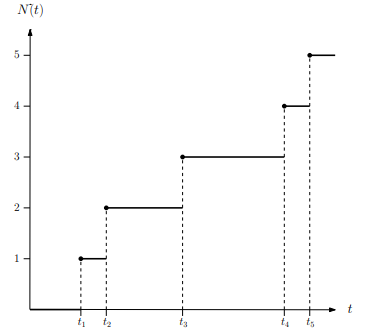
\includegraphics{PointProcessAndCountingProcess.PNG}
  	\caption{An example point process realisation $\{t_{1}, t_{2}, . . . \}$ and corresponding counting process $N(t)$.}
  	\label{PointAndCountingProcess}
  \end{figure}

To be able to fully understand what a counting process is, a point process must be defined. In this section, we introduce the fundamentals of point process. They are a foundation on which we build in later sections as the Hawkes process.

\begin{Definition}[{\cite[pp.3]{Hawkess}}(Point process)]{}	
If a sequence of random variables $T = {T_{1}, T_{2}, . . . }$, taking values in $R^{+} \cup {\infty}$, has: $P(0 < T_{0} \leq T_{1} \leq T_{2} \leq . . . ) = 1, P(T_{i} < T_{i+1}, T_{i} < \infty) = P(T_{i} < \infty) $ for $i \geq 1 $, and the number of points in a bounded region is finite almost surely (a.s.), then T is a (simple) point process.
\label{Def Point process}
\end{Definition}

The simplest point process is a Poisson process which some events arrive randomly with the constant intensity $\lambda$. This initial model describes sufficiently the simple process. For a example, the arrival of cars on a street over a short period of time. However, we need to vary the intensity event by the time $t$ to describe more complex processes such as simulating the arrivals of cars during rush hours and off-peak times. In a non-homogeneous Poisson process, the rate of event arrivals is a time function, i.e. $\lambda = \lambda(t)$.

\section{Non-homogeneous Poisson processes}
\begin{Definition}[{\cite[pp.5]{Hawkess}}(Non-homogeneous process)]{}	
Say a process $(N(t): t\geq 0)$ is a counting process and that it satisfies $ \forall s <t $ that $N(t)-N(s)$ is independent of $N(s)$ and that		
	\begin{align*}
	P(N(t + h) - N(t) = m \rvert N(t)) = 
	\begin{cases*}
	\lambda(t)h & $m = 1$ \\
	o(h) & $m > 1$  \\
	1-\lambda(t)h + o(h) & $ m = 0$  
	\end{cases*}  
	\end{align*}
then $N(t)$ is called a non-homogeneous Poisson process with $\lambda$ : $ R^{+} \rightarrow R^{+} $ called the intensity function; though if $\lambda(t) = \lambda $ for all $t \geq 0$, $N(t)$ is a homogeneous Poisson process.
\end{Definition}
However, a non-homogeneous Poisson process is only governed by an intensity function. One way to characterise a particular point process is to specify the distribution function of the next arrival time which bases on the past. The conditional intensity function is a convenient and intuitive way of specifying how the present depends on the past in an evolutionary point process.
\section{Conditional intensity functions}
\begin{Definition}[{\cite[pp.6]{Hawkess}}(Conditional intensity function)]{}	
Consider a counting process $N(.)$ with associated histories $H(.)$. If a function $\lambda^{*}(t)$ exists such that
 $$\lambda^{*}(t)= \lim_{h \to 0} \dfrac{E[N(t + h)-N(t) |H(t)]}{h}$$
that only relies on information of $N(.)$ in the past, then it is called the
conditional intensity function of $N(.)$.
\end{Definition}
 
 
	\newpage
	\chapter{Hawkes Process}
In this chapter, we introduce a class of processes in which the event arrival rate explicitly depends on past events – i.e. self-exciting processes – and we further detail the most well-known self-exciting process, the Hawkes process.
\section{Hawkes process definition}
\begin{Definition}[{\cite[pp.9]{Hawkess}}(Hawkes process definition)]{}	
	Considers $(N(t): t\in R)$ a counting process, with associated history $(H(t):
	t \in R)$, that satisfies
	\begin{align*}
	P(N(t + h) - N(t) = m \rvert N(t)) = 
	\begin{cases*}
	\lambda^{*}(t)h & $m = 1$ \\
	o(h) & $m > 1$  \\
	1-\lambda^{*}(t)h + o(h) & $ m = 0$  
	\end{cases*}  
	\end{align*}
Suppose the process’conditional intensity function is of the form
	\begin{align*}
	\lambda^{*}(t) = \lambda + \displaystyle\int\limits_{-\infty}^{t} \mu(t-u)dN(u) 
	\end{align*}
for some $\lambda \in R^{+}$ and $\mu: R^{+} \rightarrow R^{+} \cup {0}$ which are called the background intensity and excitation function respectively. Such a process $N(.)$ is a Hawkes process.
\end{Definition}

There are two major simulation approaches in the literature such as intensity-based and cluster-based, since a Hawkes process can be defined via a conditional stochastic intensity function.

\section{Intensity-based Hawkes Process Model}

\subsection{Hawkes conditional intensity function}
\begin{Definition}[{\cite[pp.10-11]{Hawkess}}(conditional intensity function)]{}	
	The observed sequence of past arrival times of the point process up to time $t$, the Hawkes conditional intensity is
	$$\lambda^{*}(t) = \lambda + \sum_{t_{i} < t} \mu (t-t_{i})$$
	In this case $\mu(.)$ is specified by constants $\alpha, \beta \in R^{+}$ such that
	\begin{align}
	\label{Def_HakessIntensity}
	\lambda^{*}(t) = &
	\lambda + \displaystyle\int\limits_{-\infty}^{t} \alpha e^{-\beta(t-s)}dN(s) 
	\\
	& = \lambda + \sum_{t_{i} < t}\alpha e^{-\beta(t-t_{i})} \nonumber
	\end{align}
	with each arrival in the system instantaneously increases the arrival intensity by $\alpha$, then over time this arrival’s influence decays at rate $\beta$.
\end{Definition}
If the Hawkes process is restricted to $R^{+}$ with
some initial condition $\lambda^{*}(0) = \lambda_{0}$ then the conditional intensity process satisfies the
stochastic differential equation
$$d\lambda^{*}(t) = \beta(\lambda - \lambda^{*}(t))dt + \alpha dN(t) , t \geq 0 .$$
	Applying stochastic calculus to yield the general solution of	
		\begin{align*}
		\lambda^{*}(t) = e^{-\beta t} (\lambda_{0} - \lambda) +\lambda + \displaystyle\int_{0}^{t} \alpha e^{\beta(t-s)}dN(s), t \geq 0. 
		\end{align*}
	which is a natural extension of Eq. \ref{Def_HakessIntensity}.
	


\subsection{Algorithm}
Ogata (1981) proposes an algorithm for the simulation of Hawkes processes. The conditional intensity $\lambda^{*}(.)$ does not have an asymptotic upper bound, however it is common for the intensity to be non-increasing in periods without any arrivals. This implies that for $t \in (T_{i}, T_{i+1}], \lambda^{*}(t) \leq \lambda^{*}(T_{i}^{+})$. So the $M$ value can be updated during each simulation. This algorithm describes Hawkes process by thinning.
\begin{breakablealgorithm}
	\caption{Generate an Hawkes process by thinning}
	\label{Alg:Hawkes_Thinning}
	\begin{algorithmic}[H] \item
		\begin{tabbing}
			INPUT:  \=
			\\
			\> $T$: the sequence of random arrival times.
			\\
			\>$\lambda(.)$: the intensity function.
			\\
			OUTPUT: 
			\\
			\> $P$: retrieve the simulated process on $ [0, T ]$.
			\\
			1.\= \textbf{Procedure} HawkesByThinning $(T,\lambda(.))$
			\\
			2.\textbf{Require}: $\lambda^{*}(t)$ non-increasing in periods of no arrivals.
			\\
			\hspace{0.5cm} $ \varepsilon \leftarrow 10^{-10}$ (some tiny value $> 0$ )
			\\
			\hspace{0.5cm} $P \leftarrow [], t \leftarrow 0.$
			\\
			3.\textbf{General routine}
			\\
			\hspace{0.5cm}\textbf{while} $t < T $ \textbf{do}
			\\
			\hspace{1cm}Find new upper bound: $M \leftarrow \lambda^{*}(t + \varepsilon)$.
			\\
			\hspace{1cm}Generate next candidate point: $E \leftarrow Exp(M)$, $ t \leftarrow t + E $
			\\
			\hspace{1cm}Keep it with some probability: $U \leftarrow Unif(0,M)$.
			\\
			\hspace{1cm}\textbf{if} $t < T$ \textbf{and} $U \leq \lambda^{*}(t) $ \textbf{then}
			\\
			\hspace{1.5cm}$P \leftarrow [P, t].$
			\\
			\hspace{1cm}\textbf{end if}
			\\
            \hspace{0.5cm}\textbf{end while}
			\\
			\hspace{0.5cm}\textbf{return} $P$
			\\
			\hspace{0.2cm}\= \textbf{End procedure}
		\end{tabbing}
	\end{algorithmic}
\end{breakablealgorithm}
\subsection{Example}

Let us simulate Hawkes process, using Algorithm \ref{Alg:Hawkes_Thinning}. For set values of $T=30, \lambda = 0.5, \alpha=0.15, \beta=1$, we obtained a Hawkes (self-exciting) process; a graph of its intensity, along with
the event times, is presented in Figure \ref{Example_Thinning}. We see that as defined an arrival (an event) causes the conditional intensity function to increase.

  \begin{figure}[H]
  	\centering
  	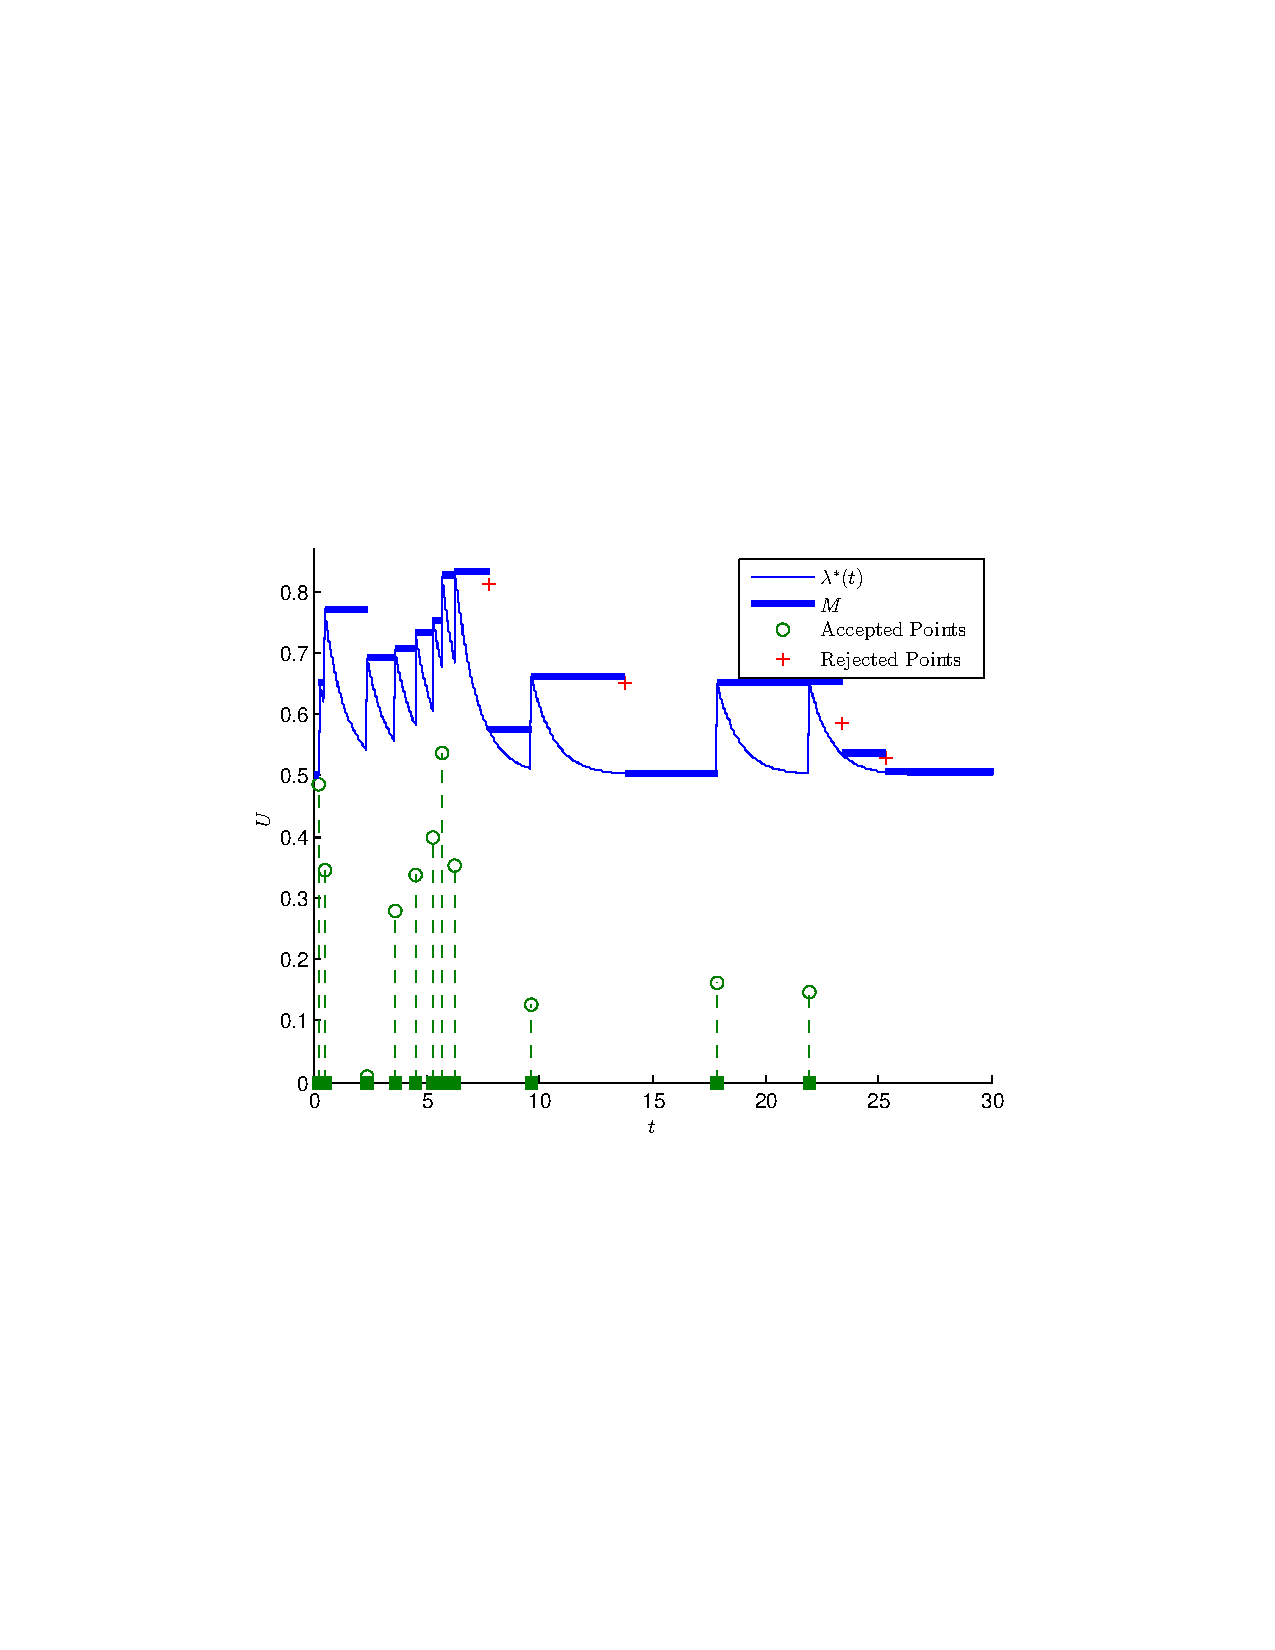
\includegraphics[trim = 0.8cm 8.5cm 0.8cm 8cm,clip,width=1.00\textwidth ]{Hawkess_Thinning.pdf}
  	\caption{A simulation of process by thinning.}
  	\label{Example_Thinning}
  \end{figure}
Figure \ref{Example_Thinning} presents A Hawkes process with $(\lambda, \alpha, \beta) =
(0.5, 0.15, 1)$. Each $(t, U)$ point describes a suggested arrival at time $t$ whose $U$ value
is given in Algorithm \ref{Alg:Hawkes_Thinning}. Plus signs signs indicate rejected points, circles accepted, and green squares the resulting point processes.

\section{Cluster-based Hawkes Process Model}

\subsection{Immigration–birth representation}
 Imagine counting the population in a country where people
 arrive either via immigration or by birth. Say that the stream of immigrants to the country form a homogeneous Poisson process at rate $\lambda$. Each person then produces zero or more children in an independent and identify distribution, the arrival of births form an non-homogeneous Poisson process.
  \begin{figure}[H]
  	\centering
  	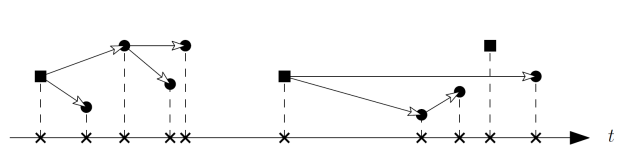
\includegraphics[width=0.8\textwidth]{Immigrate_Birth.PNG}
  	\caption{Hawkes process represented as a collection of family trees (immigration–
  		birth representation).}
 
  	\label{Immigrate_Birth}
  \end{figure}
  Squares indicate immigrants, circles are offspring/descendants, and the crosses denote the generated point process
\subsection{Algorithm}
The immigration–birth representation gives rise to a simple simulation procedure: generate the immigrant arrivals, then generate the descendants for each immigrant. This algorithm describes Hawkes process by cluster.
\begin{breakablealgorithm}
	\caption{Generate an Hawkes process by clusters}
	\label{Alg:Hawkes_clusters}
	\begin{algorithmic}[H] \item
		\begin{tabbing}
			INPUT:  \=
			\\
			\> $T$: the sequence of random arrival times.
			\\
			\>$\lambda$: the intensity function.
			\\
			\>$\alpha$, $\beta$: the constant.
			\\
			OUTPUT: 
			\\
			\> $P$:retrieve the simulated process on $ [0, T ]$.
			\\
			1.\= \textbf{Procedure} HawkesByClusters $(T,\lambda, \alpha,\beta)$
			\\
			2.\hspace{0.5cm} $P\leftarrow$ $\{\}$
			\\
			3.\hspace{0.5cm} Immigrants: $k \leftarrow Poi(\lambda T), C_{1}, C_{2}, . . . , C_{k} \xleftarrow{i.i.d} Unif(0, T)$.
			\\
			4.\hspace{0.5cm} Descendants: $D_{1}, D_{2}, . . . , D_{k}
			\xleftarrow{i.i.d} Poi(\alpha / \beta)$.
			\\
			5.\hspace{0.5cm}\textbf{for} $i \leftarrow 1 $ \textbf{to} $k$ \textbf{do}
			\\
			6.\hspace{1cm}\textbf{if} $D_{i} > 0$ \textbf{then}
			\\
			7.\hspace{1.5cm} $E_{1}, E_{2}, . . . , E_{D_{i}} 	\xleftarrow{i.i.d} Exp(\beta)$.
			\\
			8. \hspace{1.5cm} $P \leftarrow P  \cup {C_{i} + E_{1}, C_{i} + E_{2}, . . . , C_{i} + E_{D_{i}}}$.
			\\
			9.\hspace{1cm}\textbf{end if}
			\\
			10.\hspace{0.5cm}\textbf{end for}
			\\
			11.\hspace{0.5cm}Remove descendants outside $[0, T]: P \leftarrow {P_{i} : P_{i} \in P, P_{i} leq T}$.
			\\
			12.\hspace{0.5cm}Add in immigrants and sort: $P \leftarrow Sort(P \cup {C_{1}, C_{2}, . . . , C_{k}})$.
			\\
			\hspace{0.5cm}\textbf{return} $P$
			\\
			\hspace{0.2cm}\textbf{End procedure}
		\end{tabbing}
	\end{algorithmic}
\end{breakablealgorithm}

\subsection{Example}

Let us simulate Hawkes process, using Algorithm \ref{Alg:Hawkes_clusters}. For set values of $T=10, \lambda=0.89, \alpha=1, \beta=1.2$, we obtained a Hawkes process by clusters; a graph of its intensity, along with the event times, is presented in Figure \ref{Example_ClusterFamily} and \ref{Example_ClusterIntensity}. We see that as defined an arrival (an event) causes the conditional intensity function to increase.


\begin{figure}[H]
	\centering
	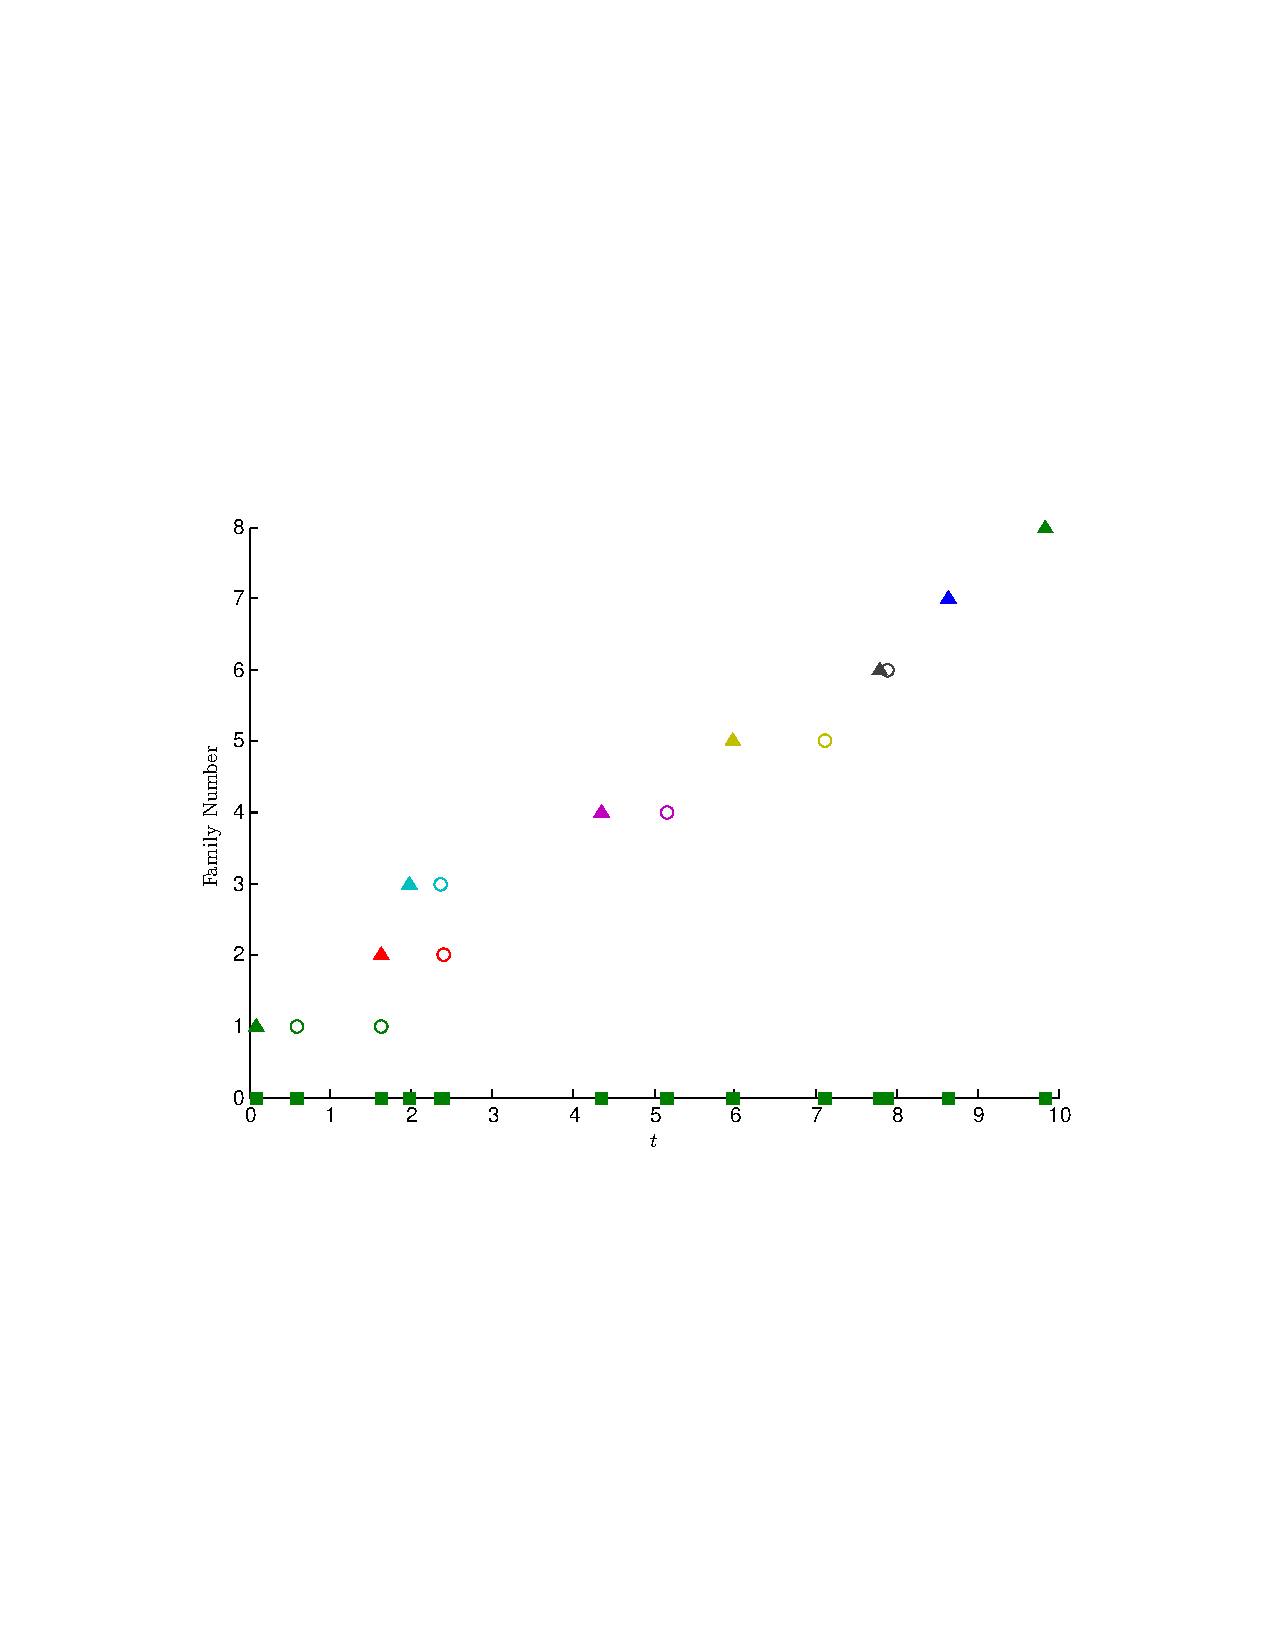
\includegraphics[trim = 0.8cm 8.5cm 0.8cm 8cm,clip,width=1.00\textwidth ]{Hawkess_ClusterFamily.pdf}
	\caption{The points generated by the immigrant–birth representation.}
	\label{Example_ClusterFamily}
\end{figure}
Figure \ref{Example_ClusterFamily} shows the
points generated by the immigrant–birth representation; it can be seen as a sequence
of vertically stacked “family trees”. The immigrant points are plotted as triangles, following circles of the same height and color are its offspring.
\begin{figure}[H]
	\centering
	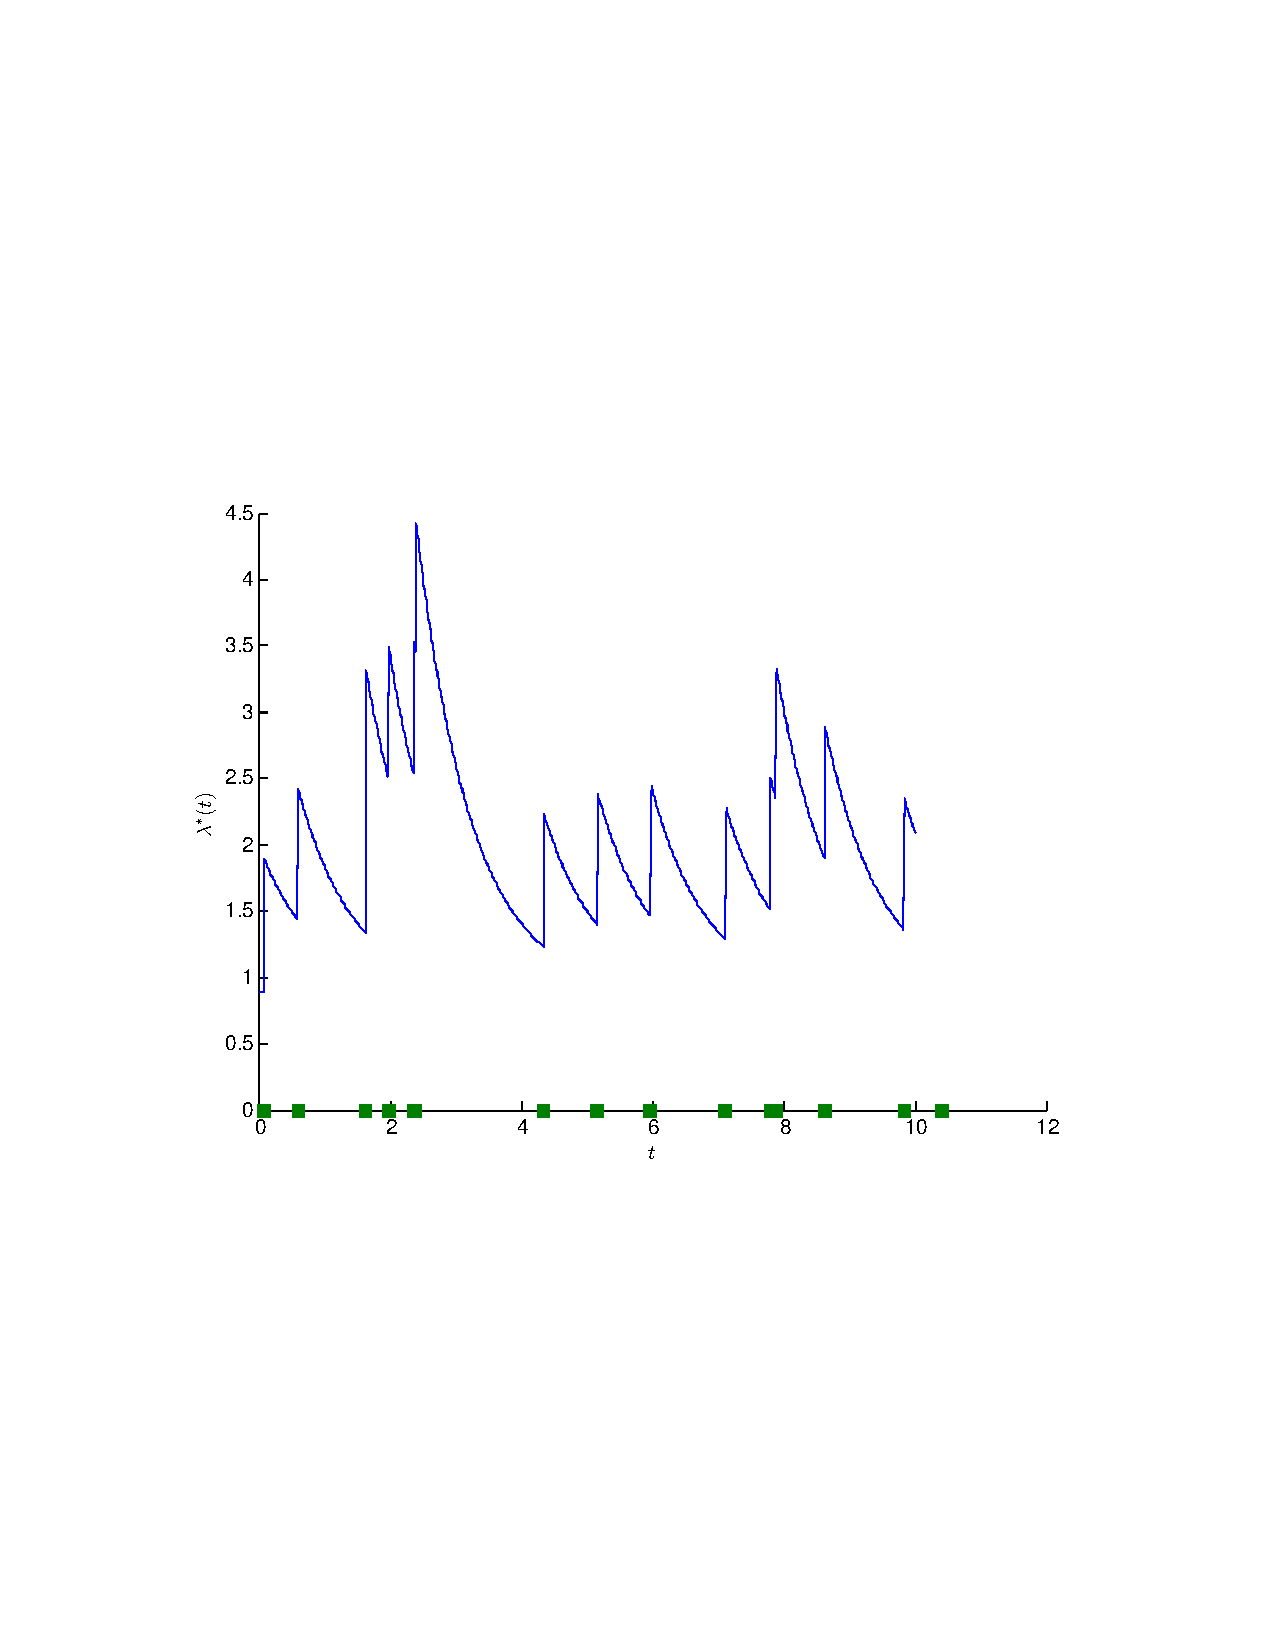
\includegraphics[trim = 0.8cm 8.5cm 0.8cm 8cm,clip,width=1.00\textwidth ]{Hawkess_ClusterIntensity.pdf}
	\caption{The intensity function.}
	\label{Example_ClusterIntensity}
\end{figure}

Figure \ref{Example_ClusterIntensity} shows the intensity function with $(\lambda, \alpha, \beta) = (0.89, 1, 1.2)$. The resulting Hawkes process arrivals are drawn as squares on the axis.  
	
	\newpage
	\chapter{Applications}
This chapter will introduced mathematically some applications which are using the Hawkes process.

\section{Seismic Events}
In reality, the earthquakes regularly occur. To decrease the risk and damage, Alan Hawkes introduced a family of probability models to the prediction of the occurrence of large earthquakes (related to the assessment of seismic risk in space and time) is complicated by the presence of clusters of aftershock. The epidemic type aftershock sequence model was introduced. This model is a particular type of marked Hawkes process for modeling earthquake times and magnitudes. the epidemic type aftershock sequence model can be defined by its intensity

$$\lambda(t) = \lambda_{0} + \alpha \sum_{t_{i} < t} e^{\delta\kappa_{i}} e^{-\beta(t-t_{i})}.$$
where $\alpha, \beta, \delta > 0 $ are parameters, with an exponential distribution as its mark density  and $\kappa_{i} \in [0, \infty)$ denotes the magnitude of an earthquake occurring
at time $t_{i}.$
$$f(\kappa|t) = \gamma e^{-\gamma\kappa}.$$
The conditional intensity function including both marks and times is
$$\lambda(t,\kappa) =( \lambda_{0} + \alpha \sum_{t_{i} < t} e^{\delta\kappa_{i}} e^{-\beta(t-t_{i})})\gamma e^{-\gamma\kappa}.$$

 \begin{figure}[H]
 	\centering
 	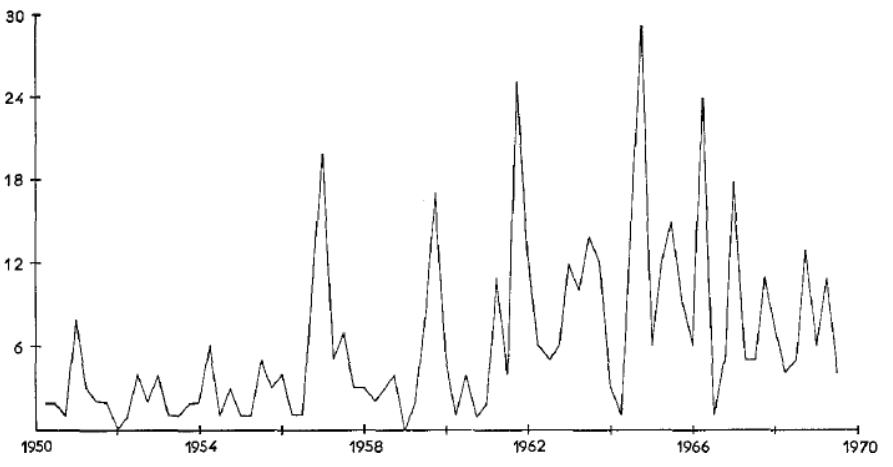
\includegraphics[width=0.8\textwidth ]{Application_Seismic.PNG}
 	\caption{The number of shocks in periods of three months for an area of the North Atlantic.}
 	\label{Application_Seismic}
 \end{figure}

Seeing in Figure \ref{Application_Seismic} that the number of shocks in periods of three months for an area of the North
Atlantic resembles the stochastic intensity function of a Hawkes process.

\section{ Risk Process with Hawkes Process}
In insurance field, the risk estimation is important. Hence Stabile and Torrisi consider risk processes with non-stationary Hawkes claims arrivals. They introduce the following risk model for the surplus process (risk process)
$$ U(t,x) = x + ct - \displaystyle\sum_{i=1}^{N^{*}(t)}Z_{i}$$
where ${N(t), t \geq 0} $is the number of points of a non-stationary Hawkes process, in the time interval $(0, t]$, $x$,$ c > 0$ and $\{Z_{i}, i = 1, 2, . . .\}$ are the same as for the classic model.

 \begin{figure}[H]
 	\centering
 	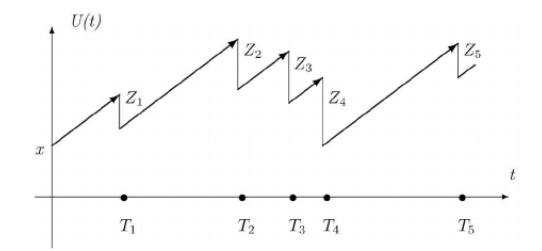
\includegraphics[width=0.8\textwidth ]{SurplusProcess.PNG}
 	\caption{Behavior of the surplus process.}
 	\label{Surplus_Process}
 \end{figure}
 The interpretation of the risk model is the following: the
 standard claims which occur according to the immigrant-points trigger claims according
 to the branching structure. Typically, the fertility rate of an immigrant is taken to
 be monotonic decreasing, meaning that the claim number process has a self -exciting
 structure in which recent events affect the intensity of claim occurrences more than
 distant ones.
  
	
%    \newpage
%    \include{Chapter5} 
	
    \newpage	
	\chapter{Conclusion}
This report provided a gentle introduction for Hawkes process. In chapter 2, we covered the key definitions such as point process, counting process, non-homogeneous Poisson process, intensity function and its properties which providing some basic knowledge about Hawkes process. In chapter 3, we introduced the definitions of Hawkes process and Hawkes conditional intensity function including Intensity-based Hawkes Process model and Cluster-based Hawkes Process model, some algorithms, examples and Matlab\textsuperscript \textregistered simulation have been also given. The goal of the above materials is to provide the fundamentals to researchers who are interested in formulating and solving application problems. So we introduced some practical applications in final chapter, it includes insurance company model and crime data for specific area.

	
	\newpage
	\include{Appendices}
	
	
    %--------------------------------------------------------------------------------%
	\renewcommand{\bibname}{References}
	\addcontentsline{toc}{chapter}{References}
	\printbibliography
	
\end{document}


